\subsubsection{Sprint goal}


\subsubsection{Backlog}
\userstory%
{Come interessato al Fantacitorio,\\Voglio vedere e poter aggiornare una sintesi dei punteggi, aggiornati settimanalmente, dei politici\\Per vedere chi sta vincendo}%
{11\\(4 frontend + 7 backend)}%
{Avere una lista di tutti i politici con i loro relativi punteggi, visualizzarne una sintesi e poter modificarla}%
{}

\userstory%
{Come interessato al Fantacitorio,\\Voglio vedere una classifica cumulativa di punteggi di ogni politico\\Per capire chi sta vincendo}%
{5\\(2 frontend + 3 backend)}%
{Visualizzare una classifica cumulativa con i punti di ogni politico in ordine decrescente}%
{}

\userstory%
{Come interessato al Fantacitorio,\\Voglio sfogliare le immagini delle squadre degli altri partecipanti\\Per vedere contro chi competo}%
{7\\(3 frontend + 4 backend)}%
{Visualizzare, in una pagina, tutte le foto delle squadre partecipanti al Fantacitorio}%
{}

\userstory%
{Come interessato al Fantacitorio,\\Voglio poter cercare un utente e vedere se partecipa o meno e mostrare la sua squadra\\Per cercare chi gioca}%
{5\\(2 frontend + 3 backend)}%
{Possibilità di cercare un utente per username e controllare se possiede una squadra, in caso affermativo mostrarla}%
{}

\userstory%
{Come giocatore di scacchi,\\Voglio che la scacchiera venga pubblicata\\In modo tale che gli utenti vedano la mossa scelta}%
{3\\(0 frontend + 3 backend)}%
{Pubblicare un tweet con la foto della scacchiera allo stato attuale}%
{}

\userstory%
{Come giocatore di scacchi,\\Voglio che gli utenti di Twitter scelgano, a maggioranza, la mossa dell'avversario\\Per avanzare nella partita}%
{4\\(1 frontend + 3 backend)}%
{Scelta di una mossa in base alla maggioranza dei voti presenti nei commenti del post pubblicato}%
{}

\userstory%
{Come spettatore de \#leredita,\\Voglio visualizzare colui/colei che ha indovinato più volte nel corso delle puntate,\\Per sapere chi è più bravo/a.}%
{5\\(2 frontend + 3 backend)}%
{Possibilità di visualizzare, giorno per giorno, una classifica con i top 5 persone con più parole indovinate}%
{}

\userstory%
{Come spettatore de \#reazioneacatena,\\Voglio visualizzare colui/colei che ha indovinato più volte nel corso delle puntate,\\Per sapere chi è più bravo/a.}%
{1\\(0 frontend + 1 backend)}%
{Possibilità di visualizzare, giorno per giorno, una classifica con i top 5 persone con più parole indovinate}%
{}

\userstory%
{Come interessato al Fantacitorio,\\Voglio visualizzare delle statistiche interessanti nella classifica\\Per vedere chi sta andando bene e chi no}%
{3\\(1 frontend + 2 backend)}%
{Mostrare statistiche interessanti nella pagina della classifica, come ad esempio “best climber”, “best average” e “best single score”}%
{}

\subsubsection{Burndown}
\begin{figure}[H]
    \centering
    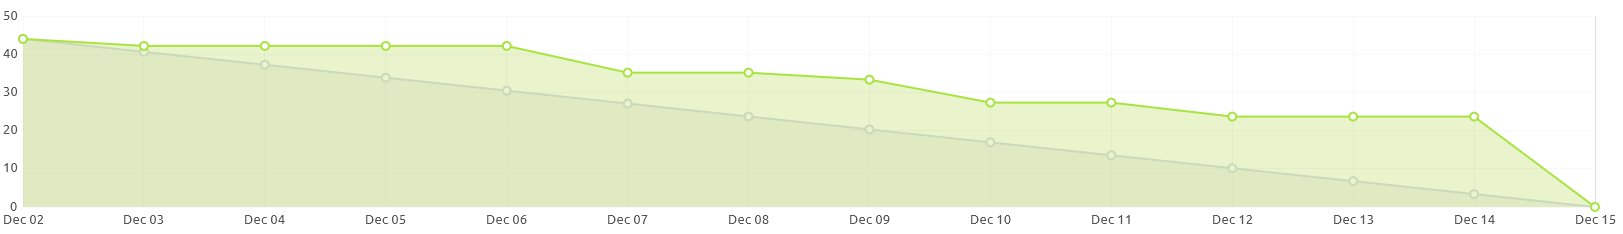
\includegraphics[width=15cm]{./img/sprint4/burndown.png}
    \caption{Burndown}
\end{figure}
\begin{figure}[H]
    \centering
    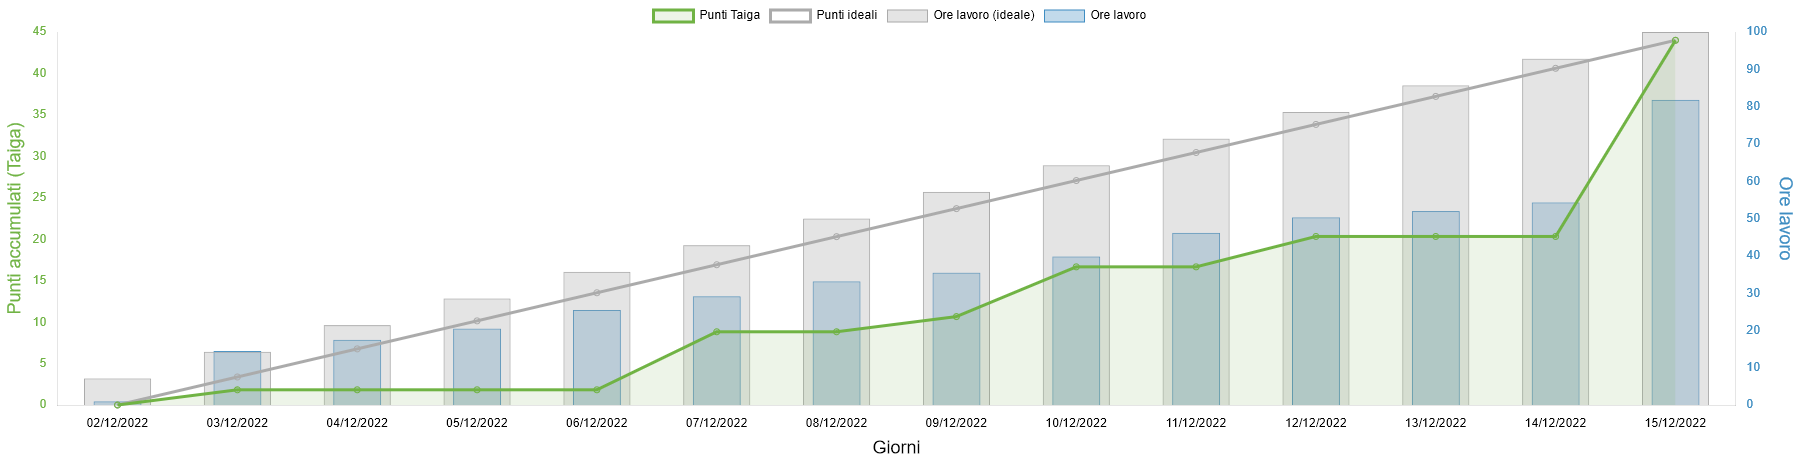
\includegraphics[width=15cm]{./img/sprint4/worktime.png}
    \caption{Progresso dei punti (asse a sinistra) e ore di lavoro (asse a destra)}
\end{figure}
\subsubsection{Retrospettiva}
\begin{figure}[H]
    \centering
    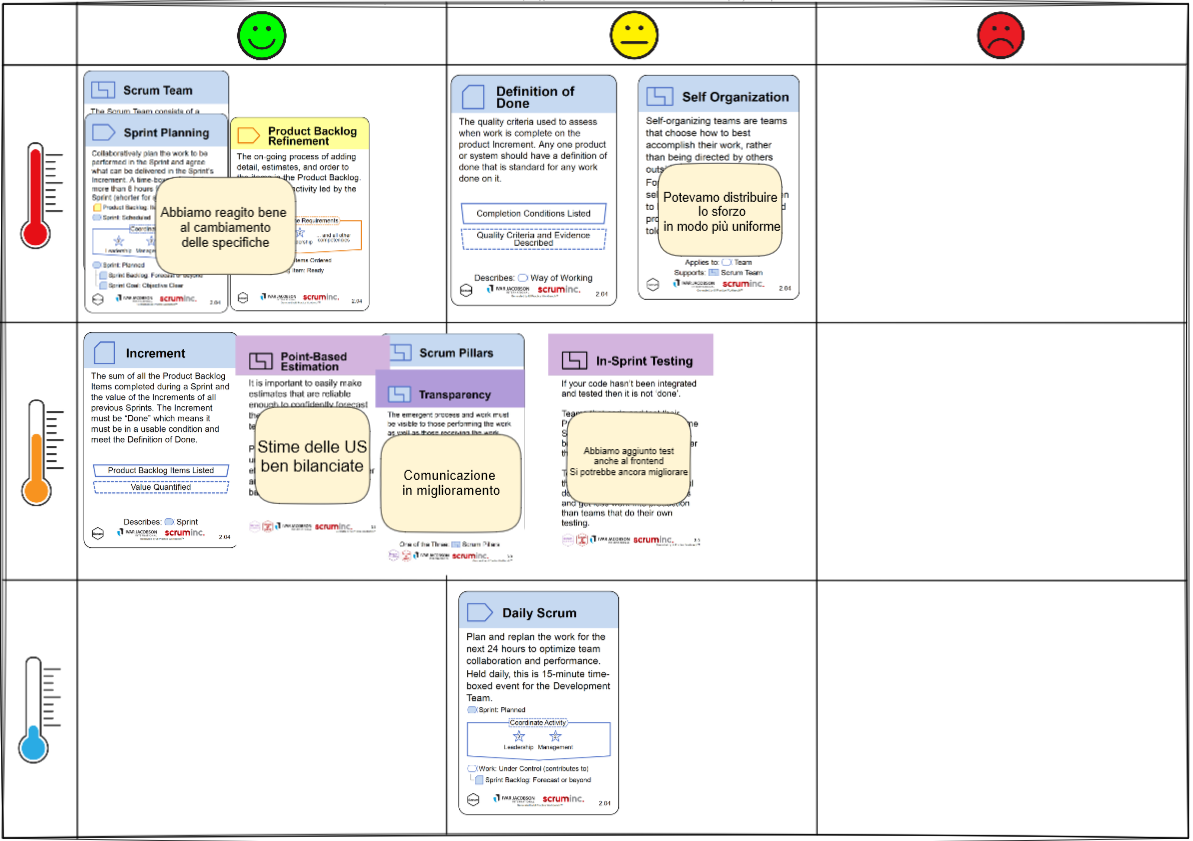
\includegraphics[width=15cm]{./img/sprint4/retrospettiva.png}
    \caption{Pre-retrospettiva del 02/12/2022}
\end{figure}